\section{EMPeror: a tool for visualizing high\hyp{}throughput microbial community data}\label{section_emperor}

\subsubsection{Background}

As microbial ecologists take advantage of high\hyp{}throughput sequencing technologies to describe microbial communities across ever\hyp{}increasing numbers of samples, new analysis tools are required to relate the distribution of microbes among larger numbers of communities, and to use increasingly rich and standards\hyp{}compliant metadata to understand the biological factors driving these relationships. In particular, the Earth Microbiome Project drives these needs by profiling the genomic content of tens of thousands of samples across multiple environment types.  

\subsubsection{Findings}

Features of EMPeror include: ability to visualize gradients and categorical data, visualize different principal coordinates axes, present the data in the form of parallel coordinates, show taxa as well as environmental samples, dynamically adjust the size and transparency of the spheres representing the communities on a per\hyp{}category basis, dynamically scale the axes according to the fraction of variance each explains, show, hide or recolor points according to arbitrary metadata including that compliant with the \gls{mixs} family of standards developed by the Genomic Standards Consortium, display jackknifed\hyp{}resampled data to assess statistical confidence in clustering, perform coordinate comparisons (useful for procrustes analysis plots), and greatly reduce loading times and overall memory footprint compared to existing approaches. Additionally, ease of sharing, given Emperor's small output file size, enables agile collaboration by allowing users to embed these visualizations via e\hyp{}mails or web pages without the need for extra plugins.

\subsubsection{Conclusions}

Here we present EMPeror, an open source and web browser enabled tool with a versatile command line interface that allows researchers to perform rapid exploratory investigations of 3D visualizations of microbial community data such as the widely used principal coordinates plots. EMPeror includes a rich set of controllers to modify features as a function of the metadata. By being specifically tailored to the requirements of microbial ecologists, EMPeror thus increases the speed with which insight can be gained from large microbiome datasets.

\subsection{Background}

Rapid increases in sequencing capacity are greatly expanding our ability to understand the microbial world: scaling from a handful of samples to hundreds, or thousands, allows a rich picture of trends over temporal and spatial scales that were previously unattainable. Human microbiome studies are not the only beneficiaries of this ability to perform increased sampling: large\hyp{}scale patterns are now being discovered in communities ranging from soils \cite{RN108} to oceans \cite{RN115} including the efforts from the \gls{icomm}.  We can now process thousands of samples in a single sequencing run \cite{RN85}, and in turn computational tools must also scale to fulfill these needs \cite{RN53}.

Although data visualization is an empowering tool that allows an efficient understanding of information \cite{RN126}, it remains a major challenge in this area of study, specifically because with more samples comes richer information relating the samples to one another (this contextual information is often referred to as `sequence metadata') and to the study design itself. When analyzing large numbers of samples, researchers need to know the patterns that link specific samples or microbes to overall patterns of diversity, and to different metadata variables: this is typically critical for usable visualizations. A well know ecological metric to quickly compare the microbial composition of the samples is beta diversity, which collates them by creating a distance matrix of these differences. Ordination methods such as \gls{pcoa} \cite{RN109} are useful for dimensionality reduction and widely used in different fields to conceptualize distance matrices, however determining how to visualize the samples to reveal clear patterns often remains a challenge. Figure~\ref{fig1} A shows the samples colored by the body site each belong to, a common approach that will make evident the main differences explained in the first two axes of variation, however when integrating metadata in the coloring patterns  (Fig~\ref{fig1} B\hyp{}1, B\hyp{}2), the plot clearly shows the age differences between the samples of an infant, compared to the samples belonging to healthy human adults.

\begin{sidewaysfigure}[htbp]
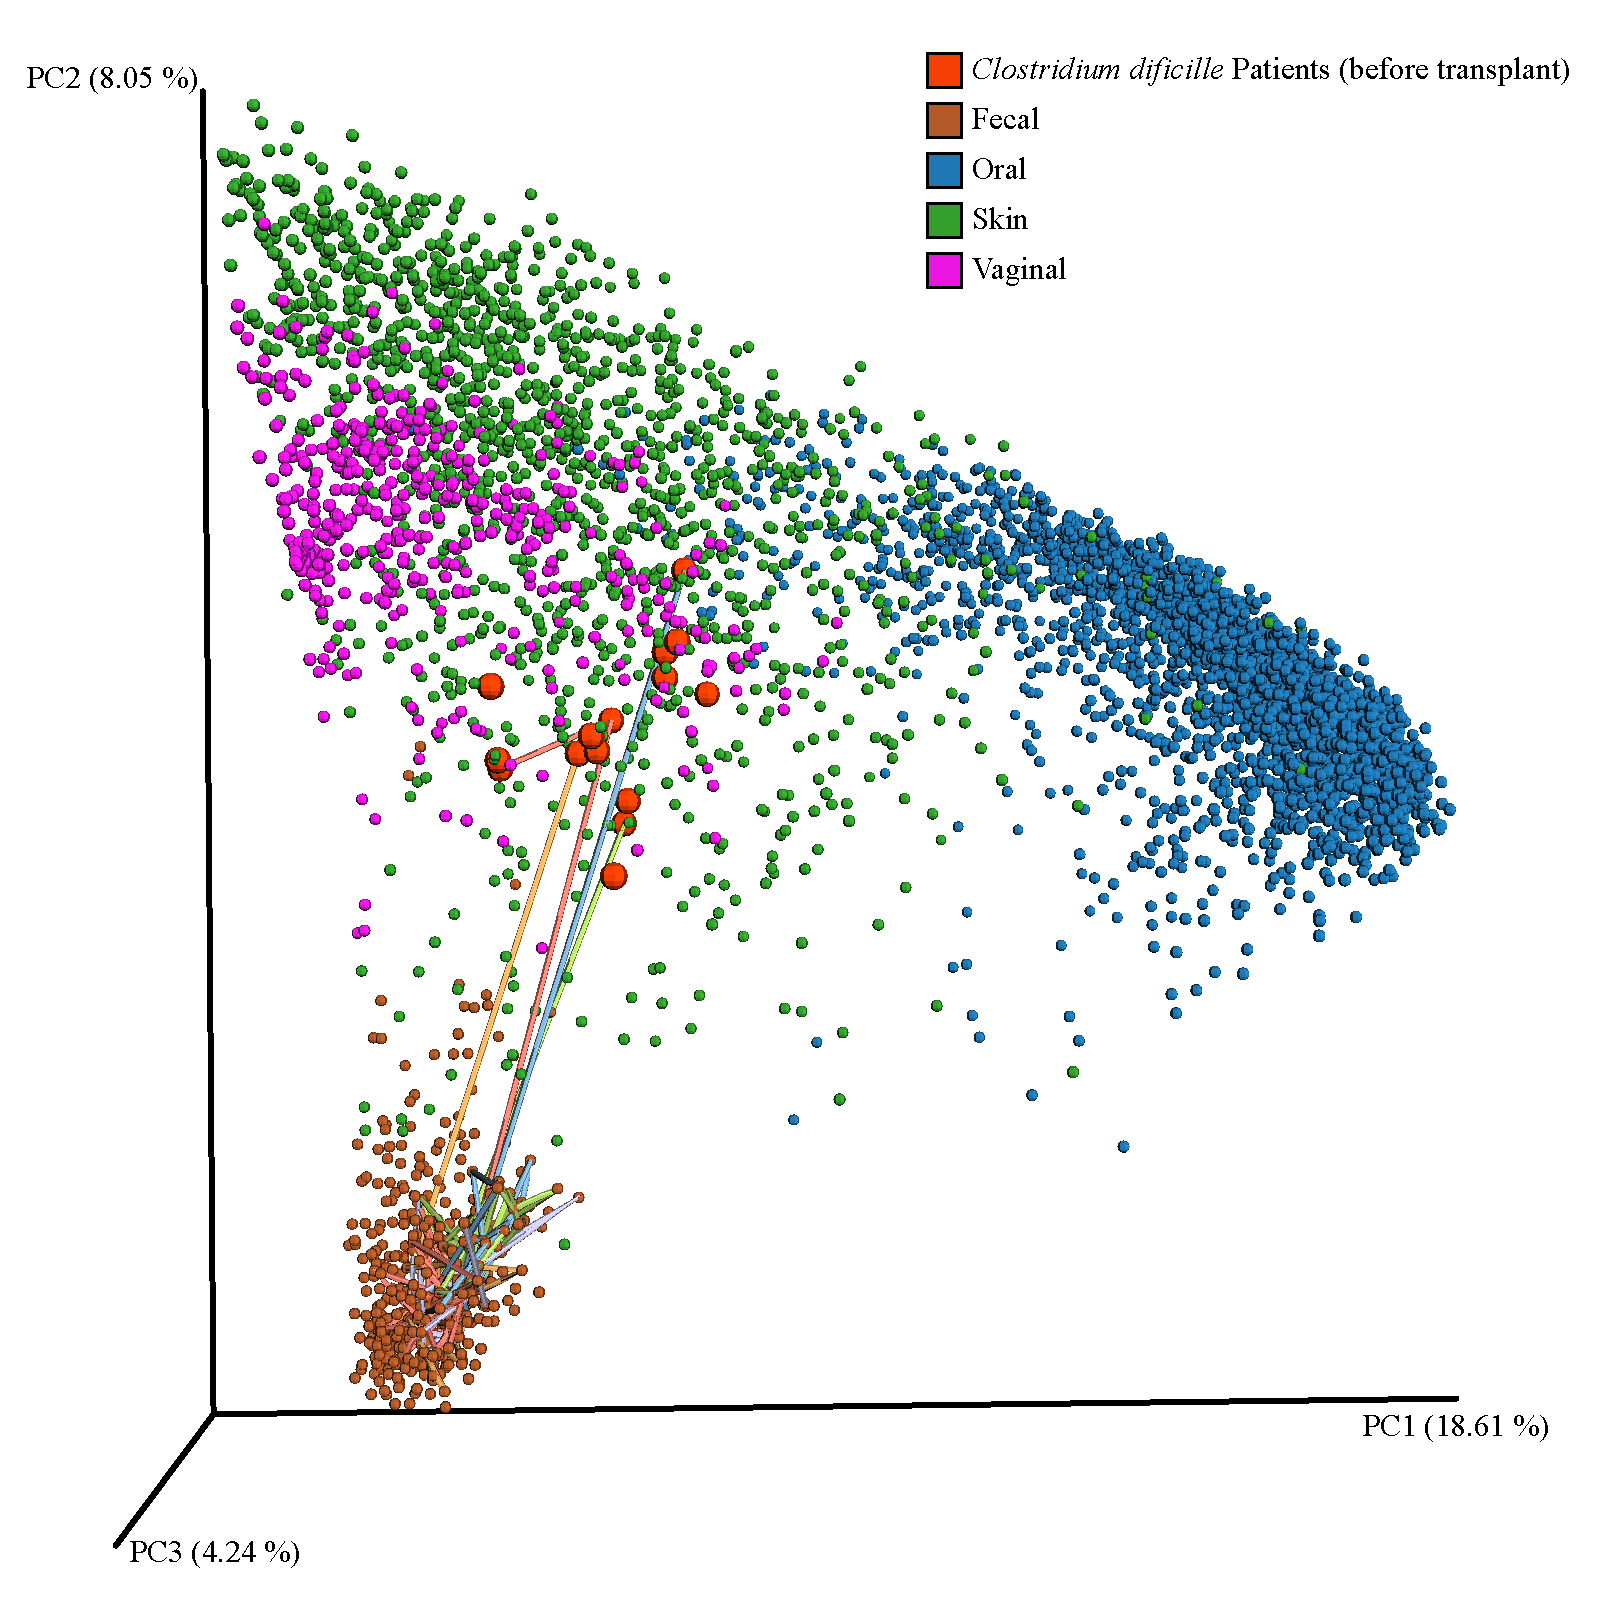
\includegraphics[width=\textheight]{emperor-figures/figure1}
\caption[EMPeror display]{EMPeror display showing the combination of the datasets described in \cite{RN85, RN4220, RN35, RN35}, consisting of 5740 samples representing human auditory canal, skin, nostril, feces, vagina, urine, hair and oral body habitats. (A) Data colored by body habitat; (B\hyp{}1) Principal coordinate 1 (PC1) vs. PC2 with the same the data colored according to the age of the subjects (a continuous variable). (B\hyp{}2) PC1 vs. an explicit time axis. The results allow us to see by immediate visual inspection that the body habitats are remarkably different between each other and that this is consistent through time as a human reaches adulthood}
\label{fig1}
\end{sidewaysfigure}

There are several existing methods for displaying \gls{pcoa} results, but none to date specifically designed to account for the common use cases in this research field; furthermore each of the most representative solutions allots different limitations. For example, \gls{qiime} \cite{RN110}, an open source framework for upstream and downstream analysis of microbial community samples generated via high\hyp{}throughput sequencing instruments, typically generates 3D plots using \gls{king} \cite{RN111} originally designed as a molecular graphics viewer, which requires static files containing each metadata field to be produced in advance, replicating the coordinates for each of these categories and resulting in long load times and large file sizes when the metadata are rich. SpotFire \cite{RN120} is a very expensive commercial solution, beyond the budget of many research laboratories. Generic packages that provide 3D plotting functionalities such as MATLAB \cite{RN121}, Mathematica \cite{RN118}, R \cite{RN117}, Excel \cite{RN119} or Matplotlib \cite{RN112} can always be used, but custom code or manual approaches are typically required to relate each point to a specific visual feature intended to highlight a given variable. Consequently, this could become a time\hyp{}consuming process, which as a side effect compromises its reliability, reusability and reproducibility. Moreover, none of the previously mentioned applications are specifically modeled to support the workflows of the modern microbial ecologist. Allowing the user to choose among metadata coloring dynamically, and separating coloring from visibility, has a surprisingly large effect in encouraging interactive exploration, understanding and analysis, and often allows insights into the main factors, as well as more subtle ones, structuring the data to be obtained much more rapidly.

\subsection{EMPEROR}
EMPeror is a thoroughly tested and open\hyp{}source software package with an interactive user interface and hardware\hyp{}accelerated graphics, implemented with \gls{html5}, \gls{webgl}, Javascript and Python, and tightly integrated with \gls{qiime} \cite{RN110} and PyCogent \cite{RN113}. EMPeror's command line interface accepts \gls{qiime} principal coordinates files and metadata mapping files, and produces an interactive 3D visualization that can be delivered in the context of a web page independent of the command line tool. As an example of EMPeror's ability to deal with continuous variables (time, alpha diversity, pH) that are part of the metadata, these factors can be integrated as an explicit axis in the plot, lines connecting subsequent points of single trajectories (treatments, subjects, sites, etc) or using a colormap to have each sample's color be a function of its position in the gradient. The main features that EMPeror provides are:
\begin{enumerate}
    \item easily change visibility features of data points in the plots based on metadata;
    \item can be easily embedded into other tools, such as Evident\footnote{\url{http://github.com/qiime/evident}} as a reusable visualization component;
    \item scale to thousands of points with minimal load times (seconds versus many minutes in \gls{king});
    \item ability to display auxiliary data to increase the understanding of the intrinsic data patterns; these include: biplots \cite{RN130}, procrustes analysis \cite{RN114}, and jackknifed beta diversity plots \cite{RN131}.
\end{enumerate}

To illustrate the effectiveness of EMPeror, we show the combination of \cite{RN85,RN4220,RN35,RN35}, see Table\ref{tab1}, as generated with the \gls{qiime} web application\footnote{\url{http://www.microbio.me/qiime/}}. This combination represents 5740 samples (spheres), and 120 columns of metadata \cite{RN132}. In \gls{king}, the resulting files for both the discrete and gradient coloring result in a size of 1.85 GB, but in EMPeror only 26 MB\footnote{\url{ftp://thebeast.colorado.edu/pub/emperor_files/}}, meaning only 1.3\% of the original size, see Figure~\ref{fig1}. Additionally, we can easily view the intrinsic age patterns within the data, Figure~\ref{fig1}~B, both panels.
EMPeror installation instructions can be found in the online documentation\footnote{\url{http://qiime.org/emperor/installation_index.html}}.


\begin{sidewaystable}[htbp]
\centering
\caption{Studies used to create Figure~\ref{fig1}}
\label{tab1}
\begin{tabular}{m{6.5cm}m{9.5cm}MM}
\toprule
Title   & General description  & Collected samples & References  \\
\midrule
Moving pictures of the human microbiome & Samples from two subjects are collected for up to 15 months in three body sites (oral, skin and gut) & 1964  & \cite{RN85,RN82} \\
\midrule
Bacterial community variation in human body habitats across space and time & Samples from   healthy adult human samples from eight subjects of up to 27 body sites & 585   & \cite{RN4220} \rule{0pt}{3ex} \\
\midrule
Structure function and diversity of the healthy human microbiome & Samples from 242 healthy adult human samples from up to eighteen different body sites & 3131  & \cite{RN35} \rule{0pt}{3ex}\\
\midrule
Succession of microbial consortia in the developing infant gut microbiome & Gut samples collected biweekly from an infant through the first 2.5 years of life  & 60  & \cite{RN35}\rule{0pt}{3ex}\\
\bottomrule
\end{tabular}
\end{sidewaystable}

\subsection{Conclusions}
EMPeror provides a user\hyp{}friendly interface and set of tools for visualizing large numbers of microbial community samples associated with increasingly extensive metadata, and interactively manipulating these data sets to add auxiliary data and visualization techniques. Additionally, it contains several user interface features, which enable straightforward modifications and customization of perceptible aspects in the plot plus the incorporation of statistical techniques, which also help increase the ease and speed of exploratory analysis. We believe that EMPeror will have a large impact on the field, especially for large\hyp{}scale environmental sampling projects such as the Earth Microbiome Project \cite{RN10}, and large\hyp{}scale clinical projects such as the Human Microbiome Project \cite{RN35}.

\subsection{Acknowledgments}

This section, in full, is a reprint of the material as it appears in ``Emperor: 
a tool for visualizing high throughput microbial community data''. Y.  
V\'azquez-Baeza, A.  Gonzalez, M. Pirrung, R.  Knight.  \emph{GigaScience}, 2, 
2013 The dissertation author was the primary investigator and author of 
this paper. In addition, we thank Jackson Chen, Jai Ram Rideout, Daniel 
McDonald, William Van Treuren, Jose Antonio Navas\hyp{}Molina, Nickolas A.  
Bokulich, Adam Robbins\hyp{}Pianka and Greg Caporaso for feedback and useful 
discussion regarding the design and implementation of the software package.  
This work was supported in part by the National Institutes of Health, the 
Crohns and Colitis Foundation of America, the Alfred P. Sloan Foundation, and 
the Howard Hughes Medical Institute. The dissertation author was the 
primary investigator and author of this paper.
